%
% File interchangeability.tex
%
\documentclass[11pt,a4paper]{article}
\usepackage[hyperref]{acl-onecolumn}
\usepackage{times}
\usepackage{latexsym}

\usepackage{url}

\usepackage[utf8]{inputenc} % allow utf-8 input
\usepackage[T1]{fontenc}    % use 8-bit T1 fonts
\usepackage{hyperref}       % hyperlinks
\usepackage{url}            % simple URL typesetting
\usepackage{booktabs}       % professional-quality tables
\usepackage{amsfonts}       % blackboard math symbols
\usepackage{nicefrac}       % compact symbols for 1/2, etc.
\usepackage{microtype}      % microtypography
\usepackage{pgfplots,pgfplotstable}
\usepackage{subcaption}

\title{Syntactic Interchangeability in Word Embedding Models \\ Supplementary Material}


\begin{document}
    \maketitle

\appendix
\section{Same-POS Neighbor Counts}\label{appendix:pos_hist}
    
    Figure~\ref{fig:nn_pos_hist} shows the the absolute number of neighbors per algorithm,
    pivot POS and neighbor POS, for all window sizes we experimented with.
    The number of nearest neighbors of the same POS is consistently decreasing with window size,
    while the number of nearest neighbors of other POS are increasing or unaffected.
    
    \begin{figure*}[h]
        \begin{subfigure}[b]{.5\textwidth}
        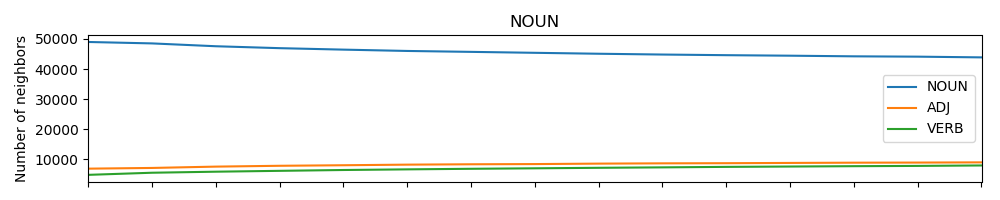
\includegraphics[width=\textwidth]{figs/NOUN_nn_100_fasttext_enwiki-20170501-clean_cbow-300d-min500_pos.png}
        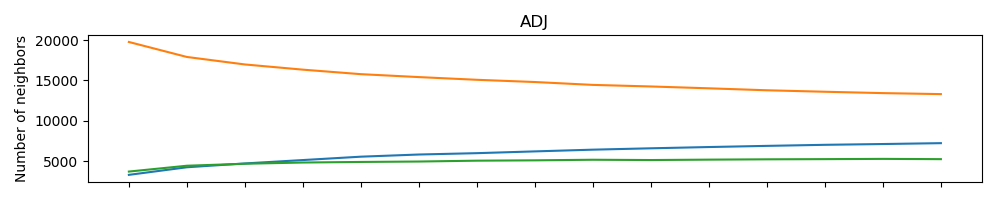
\includegraphics[width=\textwidth]{figs/ADJ_nn_100_fasttext_enwiki-20170501-clean_cbow-300d-min500_pos.png}
        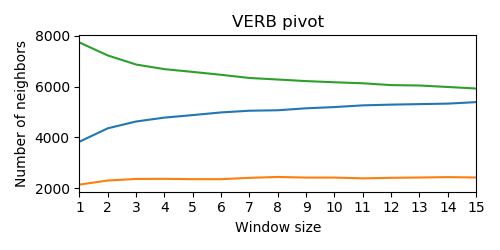
\includegraphics[width=\textwidth]{figs/VERB_nn_100_fasttext_enwiki-20170501-clean_cbow-300d-min500_pos.png}
        \caption{CBOW}
        \end{subfigure}
        \begin{subfigure}[b]{.5\textwidth}
        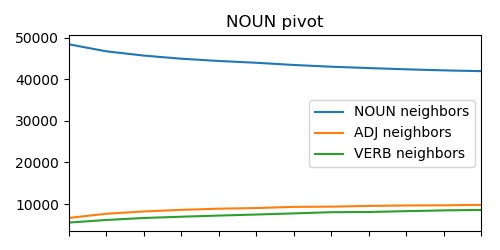
\includegraphics[width=\textwidth]{figs/NOUN_nn_100_fasttext_enwiki-20170501-clean_skipgram-300d-min500_pos.png}
        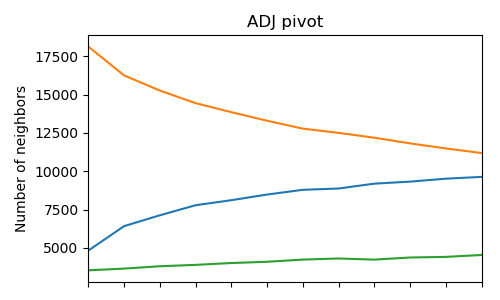
\includegraphics[width=\textwidth]{figs/ADJ_nn_100_fasttext_enwiki-20170501-clean_skipgram-300d-min500_pos.png}
        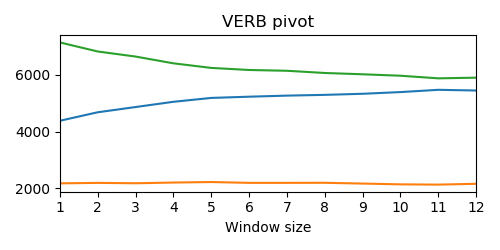
\includegraphics[width=\textwidth]{figs/VERB_nn_100_fasttext_enwiki-20170501-clean_skipgram-300d-min500_pos.png}
        \caption{SGNS}
        \end{subfigure}
        \caption{Number of neighbor per POS for each pivot POS and for each window size,
        for the CBOW~(a) and SGNS~(b) algorithms.
        The number of same-POS neighbors is consistently decreasing with window size.
        \label{fig:nn_pos_hist}}
    \end{figure*}
\end{document}
